\begin{center}
\begin{tikzpicture}
    \node (src) {};

    % pair
    \node[crossing, right=1cm of src] (0) {};
   
    % top branch
    \node[crossing, above right=1cm and 0.5cm of 0] (10) {};
    \node[gate, above right=0.25cm and 0.5cm of 10] (11) {\phantom{unit}};
    \node[gate, below right=0.25cm and 0.5cm of 10] (12) {\phantom{unit}};
    \node[pair, right=1.75cm of 10] (13) {$+$};

    \draw (10) |- (11);
    \draw (10) |- (12);
    \draw (13) |- (11);
    \draw (13) |- (12);
    \node[above right=-0.1cm and -0.1cm of 11] (label11) {$M_0$};
    \node[below right=-0.1cm and -0.1cm of 12] (label12) {$M_1$};
    \node[subcircuit, fit=(10) (11) (12) (13) (label11) (label12)] (1) {};
    \node[above right=-0.1cm and -0.1cm of 1] (label1) {$M_2$};
    % end top branch

    % bottom branch
    \node[gate, below right=1cm and 0.5cm of 0] (2) {\phantom{unit}};
    \node[above right=-0.1cm and -0.1cm of 2] (label2) {$M_3$};
    % end bottom branch

    \node[pair, right=3cm of 0] (3) {$+$};
    \draw (src) -- (0);
    \draw (0) |- (10);
    \draw (0) |- (2);
    \draw (3) |- (13);
    \draw (3) |- (2);
    \node[subcircuit, fit=(0) (1) (2) (3) (label1) (label2)] (4) {};
    \node[above right=-0.1cm and -0.1cm of 4] (label4) {$M_4$};
    % end pair

    % right gate
    \node[gate, right=1cm of 3] (5) {\phantom{unit}};
    % end right gate

    \node[above right=-0.1cm and -0.1cm of 5] (label5) {$M_5$};
    \node[right=1cm of 5] (tgt) {};

    \draw (3) -- (5);
    \draw (5) -- (tgt);
    \node[subcircuit, fit=(src) (tgt) (4) (label4)] (6) {};
    \node[above right=-0.1cm and -0.1cm of 6] (label6) {$M_6$};
\end{tikzpicture}
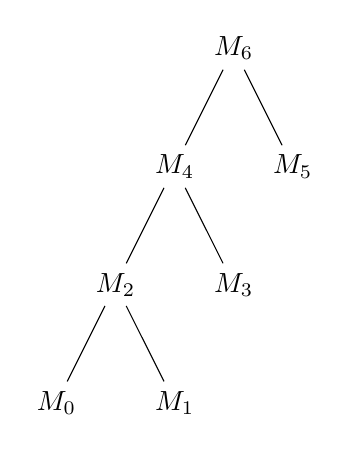
\begin{tikzpicture}
    \node {$M_6$}
        child { node {$M_4$}
            child { node {$M_2$}
                child { node {$M_0$} }
                child { node {$M_1$} }
            }
            child { node {$M_3$} }
        }
        child { node {$M_5$} };
\end{tikzpicture}
\end{center}
